\documentclass{article}

\usepackage[margin=1in]{geometry}
\usepackage{graphicx} % Allow image/pdf includes
\usepackage{extramarks} % Extra header marks (continued on next page)
\usepackage{amsmath} % Math enhancements
\usepackage{amsthm} % Theorem typesetting
\usepackage{amssymb} % Extended symbol collection
\usepackage{tikz} % Graphical element creation
\usetikzlibrary{automata,positioning}
\usepackage{algpseudocode} % Algorithm layout
\usepackage{enumitem} % Enumerate (lists)
\usepackage{ragged2e} % Alternative alignment
\usepackage{gensymb} % Generic symbols (degree, etc)
\usepackage{empheq} % Allow \boxed around \begin{empheq}
\usepackage{color,soul} % Highlighting
\usepackage{booktabs} % Enhanced table creation
\usepackage{multirow} % Table multi row
\usepackage{mathtools} % Math enhancements
\usepackage{bm} % Bold math
\usepackage[mathscr]{euscript} % Script variables
\usepackage{cancel} % Cancel through text
\usepackage{color,soul} % Highlighting
\usepackage{mathtools}
\usepackage{multirow}
\usepackage{mathrsfs}
\usepackage{physics}
\usepackage{gensymb}
\usepackage{siunitx}
\usepackage{subcaption}
\usepackage[]{algorithm2e}
\usepackage{float}
\usepackage[cache=false]{minted}
\renewcommand{\MintedPygmentize}{/Users/loganharbour/miniconda/bin/pygmentize}
\usepackage[scaled]{beramono}
\usepackage[T1]{fontenc}

\setlength\parindent{0pt} % No indents
\setlength{\parskip}{1em} % Paragraph skip

\newcommand{\vx}{\mathbf{x}} % x vector
\newcommand{\vy}{\mathbf{y}} % x vector

\newcommand{\pageTitle}{MEEN 644 - Homework 3}
\newcommand{\pageAuthor}{Logan Harbour}

\begin{document}

\title{\LARGE \textbf{\pageTitle} \vspace{-0.3cm}}
\author{\large \pageAuthor}
\date{\vspace{-0.6cm} \large \today \vspace{-0.4cm}}

\maketitle

\section*{Problem statement}

Consider a thin copper square plate of dimensions 0.5 m $\times$ 0.5 m. The temperature of the west and south edges are maintained at 50 $^\circ$C and the north edge is maintained at 100 $^\circ$C. The east edge is insulated. Using finite volume method, write a program to predict the steady-state temperature solution.

\begin{enumerate}[label=(\alph*)]
	\item \textbf{(35 points)} Set the over relaxation factor $\alpha$ from 1.00 to 1.40 in steps of 0.05 to identify $\alpha_\text{opt}$. Plot the number of iterations required for convergence for each $\alpha$.
	\item \textbf{(15 points)} Solve the same problem using $21^2, 25^2, 31^2$, and $41^2$ CVs, respectively. Plot the temperature at the center of the plate (0.25 m, 0.25 m) vs CVs.
	\item \textbf{(10 points)} Plot the steady state temperature contour in the 2D domain with the $41^2$ CV solution.
\end{enumerate}

\section*{Preliminaries}

\subsection*{Two-dimensional heat conduction}

With two-dimensional heat conduction with constant material properties, insulation on the right and prescribed temperatures on all other sides, we have the PDE
\begin{equation}
	\begin{cases}
		k \pdv{^2T}{x^2} + k \pdv{^2T}{y^2} = 0\,,\\
		T(x, 0) = T_B\,,\\
		T(0, y) = T_L\,,\\
		T(0, L_y) = T_T\,,\\
		-k \pdv{T}{x} \Big|_{x = L_x} = 0\,,
	\end{cases}
\end{equation}
where
\begin{align*}
	T_B & \equiv 50~^\circ\text{C}\,, & T_L & \equiv 50~^\circ\text{C}\,, & T_T & \equiv 100~^\circ\text{C}\,.\\
	k & \equiv 386~\text{W/m}~^\circ\text{C}\,, & L_x & \equiv 0.5~\text{m}\,, & L_y & \equiv 0.5~\text{m}\,.\\
\end{align*}

\subsection*{Control volume equations}

We discretize the region on $x \times y = [0, L_x] \times [0, L_y] = [0,L]^2$ by $N_x \times N_y = N^2$ internal nodes with $\Delta x = L_x / N_x, \Delta y =  L_y / N_y$.

Integrate over an internal control volume, $CV_\text{int}$ to obtain
\begin{align*}
	k \iint_{CV_\text{int}} \left[ \pdv{^2T}{x^2} + \pdv{^2T}{y^2} \right] dxdy & = 0\,,\\
	k \Delta y \left[ \pdv{T}{x}\Big|_e - \pdv{T}{x}\Big|_w \right] + k \Delta x \left[ \pdv{T}{y}\Big|_{n} - \pdv{T}{y}\Big|_{s} \right] & = 0\,.
\end{align*}
Now use the two node formulation for the derivative terms to obtain
\begin{equation}
	\label{eq:two_node}
	k \Delta y \left[\frac{T_{E} - T_{P}}{\delta x_e} - \frac{T_{P} - T_{W}}{\delta x_w}\right] + k \Delta x \left[ \frac{T_{N} - T_{P}}{\delta y_n} -\frac{T_{P} - T_{S}}{\delta y_s} \right] = 0\,.
\end{equation}
Note that for an internal control volume we have
\[
	\begin{cases}
		T_P = T_{i,j} \\
		T_N = T_{i,j+1} \\
		T_E = T_{i+1,j} \\
		T_S = T_{i,j-1} \\
		T_W = T_{i-1,j}
	\end{cases}\,, \qquad i = 2, 3, \ldots, N_x - 2, N_x - 1\,, \qquad j = 2, 3, \ldots, N_y - 2, N_y - 1\,,\\
\]
therefore we can represent Equation \eqref{eq:two_node} as
\[
	T_{i,j} a_p - T_{i, j+1} a_n - T_{i+1, j} a_e - T_{i, j-1} a_s - T_{i-1, j} a_w = 0\,,
\]
where (note that the below applies only to \textit{internal} control volumes)
\[
	a_n \equiv \frac{k \Delta x}{\delta y_n}\,, \quad a_e \equiv \frac{k \Delta y}{\delta x_e}\,, \quad a_s \equiv \frac{k\Delta x}{\delta y_s}\,, \quad a_w \equiv \frac{k\Delta y}{\delta x_w}\,, \quad \text{and} \quad a_p \equiv a_n + a_e + a_s + a_w\,.
\]

After studying the boundary conditions and noting that $\delta x_e = \delta x_w = \Delta x, \delta y_n = \delta y_s = \Delta y$, we can also produce the general control volume equation
\begin{multline}
	\label{eq:CV}
	T_{i,j} a_{p,i,j} - T_{i, j+1} a_{n,i,j} - T_{i+1, j} a_{e,i,j} - T_{i, j-1} a_{s,i,j} - T_{i-1, j} a_{w,i,j} = 0\,,\\ i = 1, 2, \ldots, N_x - 1, N_x\,, \quad j = 1, 2, \ldots, N_y - 1, N_y\,,
\end{multline}
where
\begin{align*}
	a_{n,i,j} & = \begin{cases}
		\frac{2 k \Delta x}{\Delta y}\,, & j = N_y \\
		\frac{k \Delta x}{\Delta y}\,, & j < N_y
	\end{cases}\,, \\
	a_{e,i,j} & = \begin{cases}
		0\,, & i = N_x \\
		\frac{k \Delta  y}{\Delta x}\,, & i < N_x
	\end{cases}\,, \\
	a_{s,i,j} & = \begin{cases}
		\frac{2 k \Delta x}{\Delta y}\,, & j = 0 \\
		\frac{k \Delta x}{\Delta y}\,, & j > 0
	\end{cases}\,, \\
	a_{w,i,j} & = \begin{cases}
		\frac{2 k \Delta y}{\Delta x}\,, & i = 0 \\
		\frac{k \Delta y}{\Delta x}\,, & i > 0
	\end{cases}\,, \\
	a_{p,i,j} & = a_{n,i,j} + a_{e,i,j} + a_{s,i,j} + a_{w,i,j}\,, \\
	T_{i, N+1} & = T_T\,, \\
	T_{N+1, j} & = 0\,, \\
	T_{i, 0} & = T_B\,, \\
	T_{0,j} & = T_L\,.
\end{align*}

\subsection*{Solving methodology}

\subsubsection*{Line-by-line method}

The problem is to be solved by the line-by-line method. In specific, the sweeping arrangement is: \textbf{south to north, west to east, north to south, east to west}. In this method, the contribution from one direction in a given control volume is lagged and moved to the right hand side in order to solve a tri-diagonal system. In the iteration process, the initial guess is the average of the Dirichlet boundary values, $(T_B + T_L + T_T) / 3$.

To define the systems solved for each sweep, we first define $a_{x,i,j}$ as $a_x$ for control volume $(i, j)$. For example, $a_{p, i, j}$ is $a_p$ for control volume $(i, j)$. Secondly, $\ell$ is the iteration index. For example, $T_{i,j}^\ell$ is the temperature solution for control volume $(i, j)$ at iteration $\ell$.

After a single solve has been made in a sweep, its solution is updated in the global solution such that the next solves have access to the latest values on the right hand side as necessary.

\subsubsection*{South to north sweep}

\def\arraystretch{1.4}

First, define the left hand side matrix for mesh row $j$ as
\begin{equation}
	\label{eq:lhs_j}
	\mathbf{A}_{s\to n, j} =
	\begin{bmatrix}
		a_{p,1,j} & a_{e,1,j} \\
		a_{w,2,j} & a_{p,2,j} & a_{e,2,j} \\
		& a_{w,3,j} & a_{p,3,j} & a_{e,3,j} \\
		& & \ddots & \ddots & \ddots \\
		& & &  a_{w, N_x - 2, j} & a_{p, N_x - 2, j} & a_{e, N_x - 2, j} \\
		& & & & a_{w, N_x - 1, j} & a_{p, N_x - 1, j} & a_{e, N_x - 1, j} \\
		& & & & & a_{w, N_x, j} & a_{p, N_x, j} \\
	\end{bmatrix}\,,
\end{equation}
and define the solution vector for mesh row $j$ as
\begin{equation}
	\label{eq:rhs_j}
	\vec{T}_{s\to n, j} =
	\begin{bmatrix}
		T_{1, j}^{\ell + 1} \\
		T_{2, j}^{\ell + 1} \\
		T_{3, j}^{\ell + 1} \\
		\vdots \\
		T_{N_x - 2, j}^{\ell + 1} \\
		T_{N_x - 1, j}^{\ell + 1} \\
		T_{N, j}^{\ell + 1}
	\end{bmatrix}\,.
\end{equation}

The first solve of a south to north sweep is of the following system along the first mesh row:
\begin{equation}
	\label{eq:south_north_1}
	\mathbf{A}_{s\to n, 1} \vec{T}_{s\to n, 1} = 
	\begin{bmatrix}
		a_{n,1,1} T_{1, 2}^\ell + a_{s,1,1} T_B + a_{w,1,1} T_L \\
		a_{n,2,1} T_{2, 2}^\ell + a_{s,2,1} T_B \\
		a_{n,3,1} T_{3, 2}^\ell + a_{s,3,1} T_B \\
		\vdots \\
		a_{n,N_x - 2,1} T_{N_x - 2, 2}^\ell + a_{s,N_x - 2,1} T_B \\
		a_{n,N_x - 1,1} T_{N_x - 1, 2}^\ell + a_{s,N_x - 1,1} T_B \\
		a_{n,N_x,1} T_{N_x, 2}^\ell + a_{s,N_x,1} T_B \\
	\end{bmatrix}\,.
\end{equation}
The next set of solves is of the following system for each mesh row $j$ from $2$ to $N_y - 1$:
\begin{equation}
	\label{eq:south_north_2}
	\mathbf{A}_{s\to n, j} \vec{T}_{s\to n, j} = 
	\begin{bmatrix}
		a_{n,1,j} T_{1, j + 1}^\ell + a_{s,1,j} T_{1, j - 1}^\ell + a_{w,1,j} T_L \\
		a_{n,2,j} T_{2, j + 1}^\ell + a_{s,2,j} T_{2, j - 1}^\ell \\
		a_{n,3,j} T_{3, j + 1}^\ell + a_{s,3,j} T_{3, j - 1}^\ell \\
		\vdots \\
		a_{n,N_x - 2,j} T_{N_x - 2, j+1}^\ell + a_{s,N_x - 2,j} T_{N_x - 2, j - 1}^\ell \\
		a_{n,N_x - 1,j} T_{N_x - 1, j+1}^\ell + a_{s,N_x - 1,j} T_{N_x - 1, j - 1}^\ell \\
		a_{n,N_x,j} T_{N_x, j+1}^\ell + a_{s,N_x,j} T_{N_x, j - 1}^\ell \\
	\end{bmatrix}\,, \quad \forall ~ j = 2, \ldots, N_y - 1\,.
\end{equation}
The last solve of a south to north sweep is of the following system along the last mesh row:
\begin{equation}
	\label{eq:south_north_3}
	\mathbf{A}_{s\to n, N_y} \vec{T}_{s\to n, N_y} = 
	\begin{bmatrix}
		a_{n,1,N_y} T_T + a_{s,1,N_y} T_{1, N_y - 1} + a_{w,1,N_y} T_L \\
		a_{n,2,N_y} T_T + a_{s,2,N_y} T_{2, N_y - 1} \\
		a_{n,3,N_y} T_T + a_{s,3,N_y} T_{3, N_y - 1} \\
		\vdots \\
		a_{n,N_x - 2,N_y} T_T + a_{s,N_x - 2,1} T_{N_x - 2, N_y - 1} \\
		a_{n,N_x - 1,N_y} T_T + a_{s,N_x - 1,1} T_{N_x - 1, N_y - 1} \\
		a_{n,N_x,N_y} T_{N_x, 2}^\ell + a_{s,N_x,1} T_{N_x, N_y - 1} \\
	\end{bmatrix}\,.
\end{equation}

\subsubsection*{East to west sweep}

Similarly, define the left hand side matrix for mesh column $i$ as
\begin{equation}
	\label{eq:lhs_i}
	\mathbf{A}_{e\to w, i} =
	\begin{bmatrix}
		a_{p,i,1} & a_{n,i,1} \\
		a_{s,i,2} & a_{p,i,2} & a_{n,i,2} \\
		& a_{s,i,3} & a_{p,i,3} & a_{n,i,3} \\
		& & \ddots & \ddots & \ddots \\
		& & &  a_{s, i, N_y - 2} & a_{p, i, N_y - 1} & a_{n, i, N_y - 1} \\
		& & & & a_{s, i, N_y - 1} & a_{p, i, N_y - 1} & a_{n, i, N_y - 1} \\
		& & & & & a_{s, i, 1} & a_{p, i, N_y} \\
	\end{bmatrix}\,,
\end{equation}
and define the solution vector for mesh column $i$ as
\begin{equation}
	\label{eq:rhs_i}
	\vec{T}_{e\to w, i} =
	\begin{bmatrix}
		T_{i, 1}^{\ell + 1} \\
		T_{i, 2}^{\ell + 1} \\
		T_{i, 3}^{\ell + 1} \\
		\vdots \\
		T_{i, N_y - 2}^{\ell + 1} \\
		T_{i, N_y - 1}^{\ell + 1} \\
		T_{i, N_y}^{\ell + 1}
	\end{bmatrix}\,.
\end{equation}

The first solve of a east to west sweep is of the following system along the first mesh column:
\begin{equation}
	\label{eq:east_west_1}
	\mathbf{A}_{e\to w, 1} \vec{T}_{e\to w, 1} = 
	\begin{bmatrix}
		a_{w,1,1} T_L + a_{e, 1, 1} T_{2, 1}^\ell + a_{s, 1, 1} T_B \\
		a_{w,1,2} T_L + a_{e, 1, 2} T_{2, 2}^\ell \\
		a_{w,1,3} T_L + a_{e, 1, 3} T_{2, 3}^\ell\\
		\vdots \\
		a_{w,1,N_y - 2} T_L + a_{e, 1, N_y - 2} T_{2, N_y - 2}^\ell \\
		a_{w,1,N_y - 1} T_L + a_{e, 1, N_y - 1} T_{2, N_y - 1}^\ell\\
		a_{w,1,N_y} T_L +  a_{e, 1, N_y} T_{2, N_y}^\ell + a_{n, 1, N_y} T_T \\
	\end{bmatrix}\,.
\end{equation}
The next set of solves is of the following system for each mesh column $i$ from $2$ to $N_x - 1$:
\begin{equation}
	\label{eq:east_west_2}
	\mathbf{A}_{e\to w, i} \vec{T}_{e\to w, i} = 
	\begin{bmatrix}
		a_{w,i,1} T_{i-1, 1}^\ell + a_{e, i, 1} T_{i+1, 1}^\ell + a_{s, i, 1} T_B \\
		a_{w,i,2} T_{i-1, 2}^\ell + a_{e, i, 2} T_{i+1, 2}^\ell \\
		a_{w,i,3} T_{i-1, 3}^\ell + a_{e, i, 3} T_{i+1, 3}^\ell\\
		\vdots \\
		a_{w,i,N_y - 2} T_{i-1, N_y - 2}^\ell + a_{e, i, N_y - 2} T_{i+1, N_y - 2}^\ell \\
		a_{w,i,N_y - 1} T_{i-1, N_y - 1}^\ell + a_{e, i, N_y - 1} T_{i+1, N_y - 1}^\ell\\
		a_{w,i,N_y} T_{i-1, N_y}^\ell + a_{e, i, N_y} T_{i+1, N_y}^\ell + a_{n, i, N_y} T_T \\
	\end{bmatrix}\,, \quad \forall ~ i = 2, \ldots, N_x - 1\,.
\end{equation}
The last solve of a south to north sweep is of the following system along the last mesh column:
\begin{equation}
	\label{eq:east_west_3}
	\mathbf{A}_{e\to w, N_x} \vec{T}_{e\to w, N_x} = 
	\begin{bmatrix}
		a_{w,N_x,1} T_{N_x-1, 1}^\ell + a_{s, N_x, 1} T_B \\
		a_{w,N_x,2} T_{N_x-1, 2}^\ell \\
		a_{w,N_x,3} T_{N_x-1, 3}^\ell \\
		\vdots \\
		a_{w,N_x,N_y - 2} T_{N_x-1, N_y - 2}^\ell \\
		a_{w,N_x,N_y - 1} T_{N_x-1, N_y - 1}^\ell \\
		a_{w,N_x,N_y} T_{N_x-1, N_y}^\ell + a_{n, N_x, N_y} T_T \\
	\end{bmatrix}\,.
\end{equation}

\subsubsection*{North to south sweep}

The north to south sweep is the same as the south to north sweep, except the systems are solved in backwards order. The order is then mesh rows $[N_y, N_y - 1, N_y - 2, \ldots, 2, 1]$.

\subsubsection*{West to east sweep}

The west to east sweep is the same as the east to west sweep, except in backwards order. The order is then mesh columns $[N_x, N_x - 1, N_x - 2, \ldots, 2, 1]$.

\subsubsection*{Convergence}

The solve is checked for convergence after all four sweeps (south to north, west to east, north to south, and east to west) have completed. The criteria is
\begin{equation}
	R = \sum_\text{CV} \left| a_p T_p - \sum_{\text{nb}} a_\text{nb} T_\text{nb} b_p\right|\leq 10^{-5}\,.
\end{equation}

\subsubsection*{Relaxation}

Upon solving an individual system $Ax^{\ell + 1} = b$ with relaxation (where $\ell$ is the iteration index, i.e., $x^\ell$ is the solution from the previous iteration), the system is relaxed with the coefficient $\alpha$ by modifying it after construction by
\[
	\begin{cases}
		a_{ii} = a_{ii} \alpha^{-1}\,,\\
		b_i = b_i + (\alpha^{-1} - 1) a_{ii} x_i^\ell\,,
	\end{cases} \quad i = 1, \ldots, N\,,
\]
and it is then solved using the standard TDMA algorithm.

\section*{Results}

\subsection*{Part a}

With the given range of $\alpha$, it was determined for this specific problem with $15^2$ CVs that $\alpha_\text{opt} \approx 1.3$ (given that it required the fewest iterations). The solve did not converge (with an attempted 2,000 iterations) for $\alpha = 1.4$. The requested figure showing the residuals follows in Figure \ref{fig:a}.

\begin{figure}[H]
	\centering
	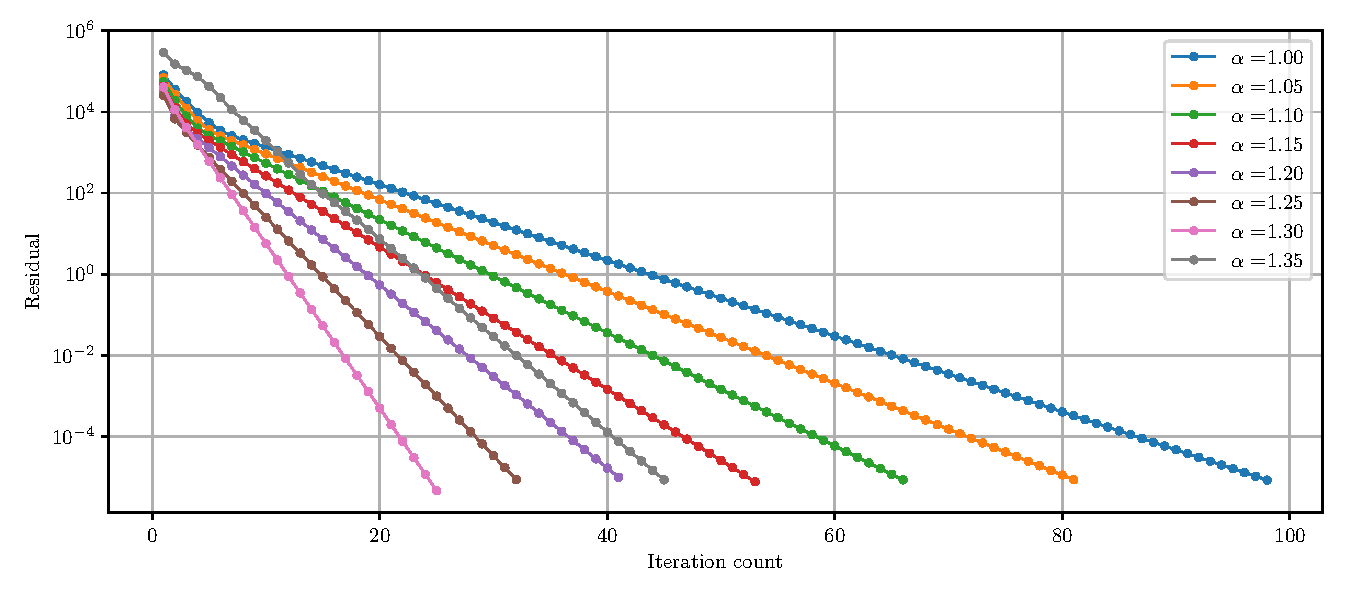
\includegraphics[width=\linewidth]{../results/a}
	\caption{Plot of the residual vs. iteration count for each relaxation parameter, $\alpha$.}
	\label{fig:a}
\end{figure}

\subsection*{Part b}

With a mesh refinement of $21^2, 25^2, 31^2,$ and $41^2$ CVs, the center temperature for each refinement with varying relaxation parameter $\alpha$ is plotted below in Figure \ref{fig:b-temps}. The same result is tabulated in Table \ref{table:b-temps}. Note the fact that to 6 digits the solution does not change for a given refinement with a change in $\alpha$. This is due to the fact that (providing the scheme converges to within the desired tolerance) relaxation will not change the solution significantly (to within the tolerance).

\begin{figure}[H]
	\centering
	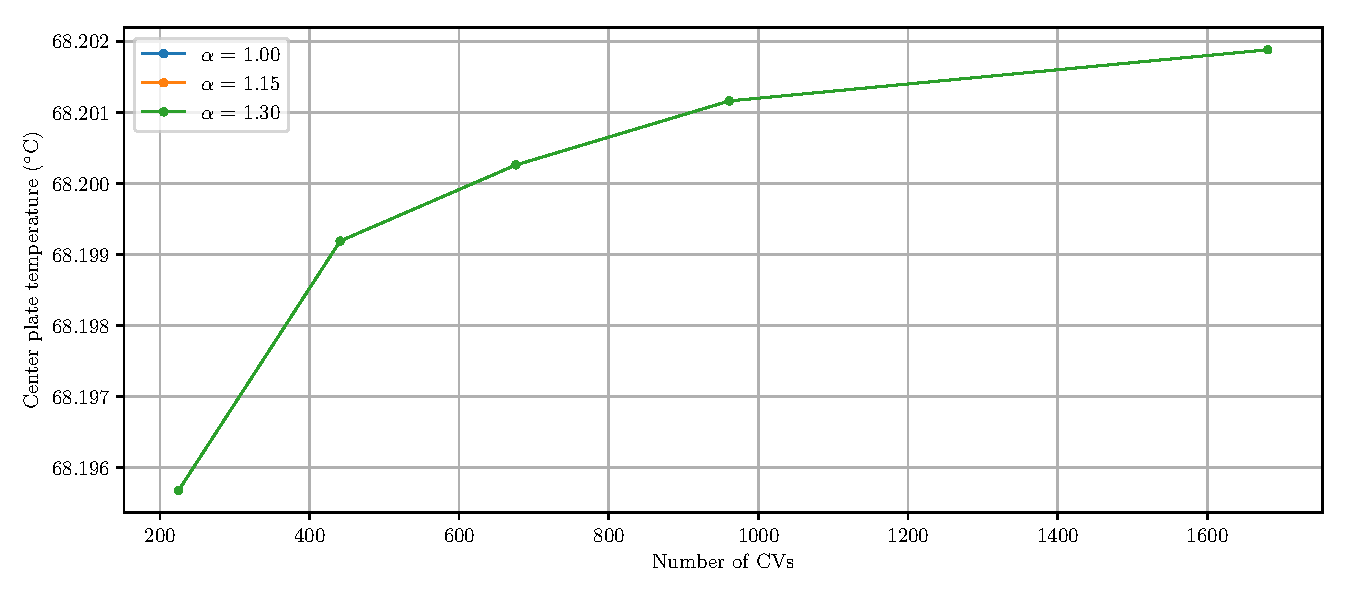
\includegraphics[width=\linewidth]{../results/b-temps}
	\caption{Plot of the center temperature with mesh refinement.}
	\label{fig:b-temps}
\end{figure}

\def\arraystretch{1.3}
\begin{table}[H]
	\small
	\centering
	\caption{The center temperature with varying refinements and relaxation parameters.}
	\vspace{0.2cm}
	\begin{tabular}{c|c|c|c}
		\multirow{2}{*}{CVs} & \multicolumn{3}{c}{Center temperature ($^\circ$C)} \\
		\cline{2-4}
		& $\alpha = 1.0$ & $\alpha = 1.15$ & $\alpha = 1.30$ \\     
		\hline
		225  & 68.19568 & 68.19568 & 68.19568 \\
		441  & 68.19919 & 68.19919 & 68.19919 \\
		625  & 68.20026 & 68.20026 & 68.20026 \\
		961  & 68.20116 & 68.20116 & 68.20116 \\
		1681 & 68.20188 & 68.20188 & 68.20188
	\end{tabular}
	\label{table:b-temps}
\end{table}

With refinement, the residuals were plotted below in Figure \ref{fig:b-iterations}. No refinement levels for $21^2$ CVs and above converged for $\alpha = 1.35, 1.4$ with 2,000 maximum iterations.

\begin{figure}[H]
	\centering
	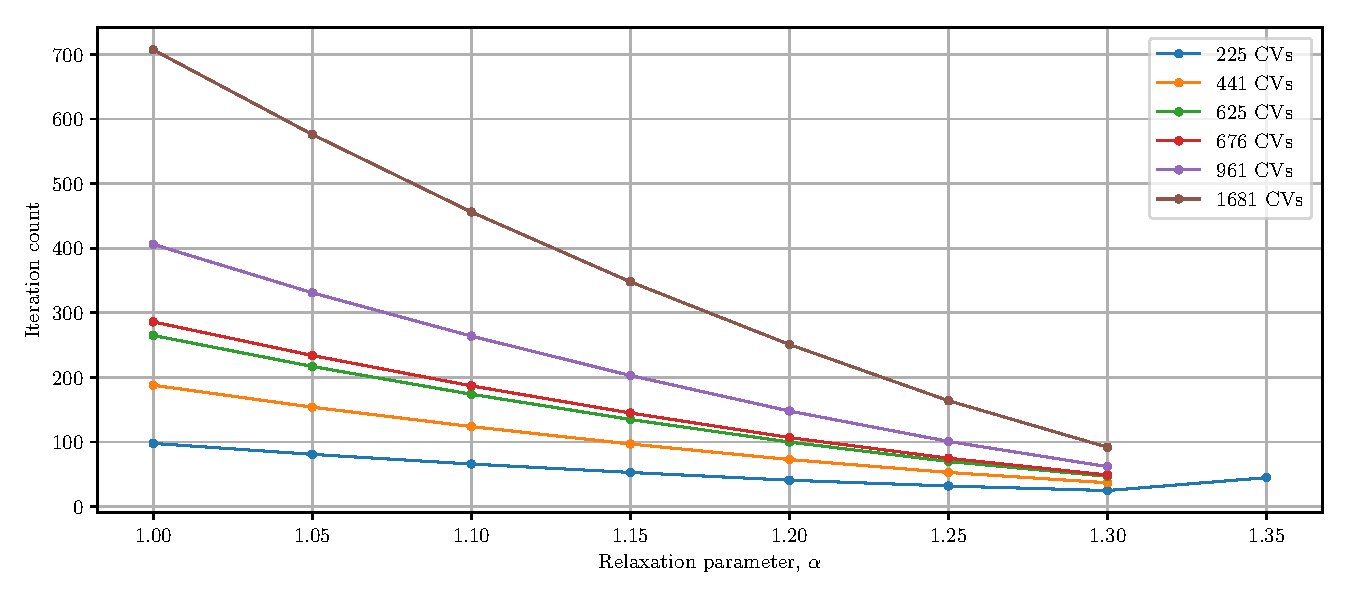
\includegraphics[width=\linewidth]{../results/b-iterations}
	\caption{Plot of the residual vs. iteration count for the more refined problems.}
	\label{fig:b-iterations}
\end{figure}

\subsection*{Part c}

With the final mesh refinement of $41^2$ CVs and $\alpha = 1$, a colored contour plot of the temperature solution follows in Figure \ref{fig:c}.

\begin{figure}[H]
	\centering
	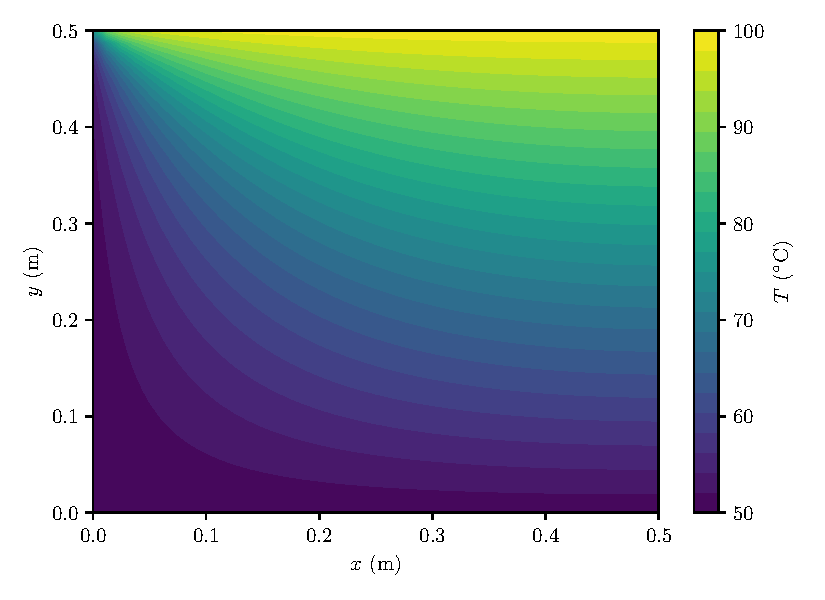
\includegraphics[width=0.7\linewidth]{../results/c}
	\caption{Plot of the solution with $41^2$ CVs.}
	\label{fig:c}
\end{figure}

\section*{Code listing}

For the implementation, we have the following files:
\begin{itemize}
	\item \texttt{Makefile} -- Allows for compiling the c++ project with \texttt{make}.
	\item \texttt{hwk3.cpp} -- Contains the \texttt{main()} function that is required by C that runs the cases requested in this problem set.
	\item \texttt{Conduction2D.h} / \texttt{Conduction2D.cpp} -- Contains the \texttt{Conduction2D} class which is the solver for the 2D heat conduction problem required in this homework.
	\item \texttt{Matrix.h} -- Contains the \texttt{Matrix} class which provides storage for a matrix with various standard matrix operations.
	\item \texttt{TriDiagonal.h} -- Contains the \texttt{TriDiagonal} class which provides storage for a tri-diagonal matrix including the TDMA solver found in the member function \texttt{solveTDMA()}.
	\item \texttt{plots.py} - Produces the plots in this report.
\end{itemize}

\subsection*{Makefile}
\inputminted[fontsize=\footnotesize]{Makefile}{../Makefile}

\subsection*{hwk3.cpp}
\inputminted[fontsize=\footnotesize]{c++}{../hwk3.cpp}

\subsection*{Conduction2D.h}
\inputminted[fontsize=\footnotesize]{c++}{../Conduction2D.h}

\subsection*{Conduction2D.cpp}
\inputminted[fontsize=\footnotesize]{c++}{../Conduction2D.cpp}

\subsection*{Matrix.h}
\inputminted[fontsize=\footnotesize]{c++}{../Matrix.h}

\subsection*{TriDiagonal.h}
\inputminted[fontsize=\footnotesize]{c++}{../TriDiagonal.h}

\subsection*{plots.py}
\inputminted[fontsize=\footnotesize]{python}{../plots.py}

\end{document}
